
\documentclass[fleqn,addpoints]{exam}
\usepackage{amsmath}
\usepackage{graphicx}
\usepackage{float}

% \printanswers

\title{Math 115 Practice Problems}
\date{October 12, 2010}

\begin{document}

\maketitle

\section{Linear Equations}

\begin{questions}

\question 
Find the slope of the line through $(1, 2)$ and $(-2, 4)$.
\vspace{4cm}

\question
Find the equation of the line parallel to $y(x)=2x+3$ and through $(-1, 1)$.
\vspace{5cm}

\question
Find the equation of the line perpendicular to $y(x)=2x+3$ and through $(-1, 1)$.
\vspace{5cm}

\pagebreak

\section{Graphing}

\question 
The following graphs are all rigid transformations of $f(x) = x^3$.  For each graph, find the function which produced it.

\begin{center}
\begin{figure}[H]
  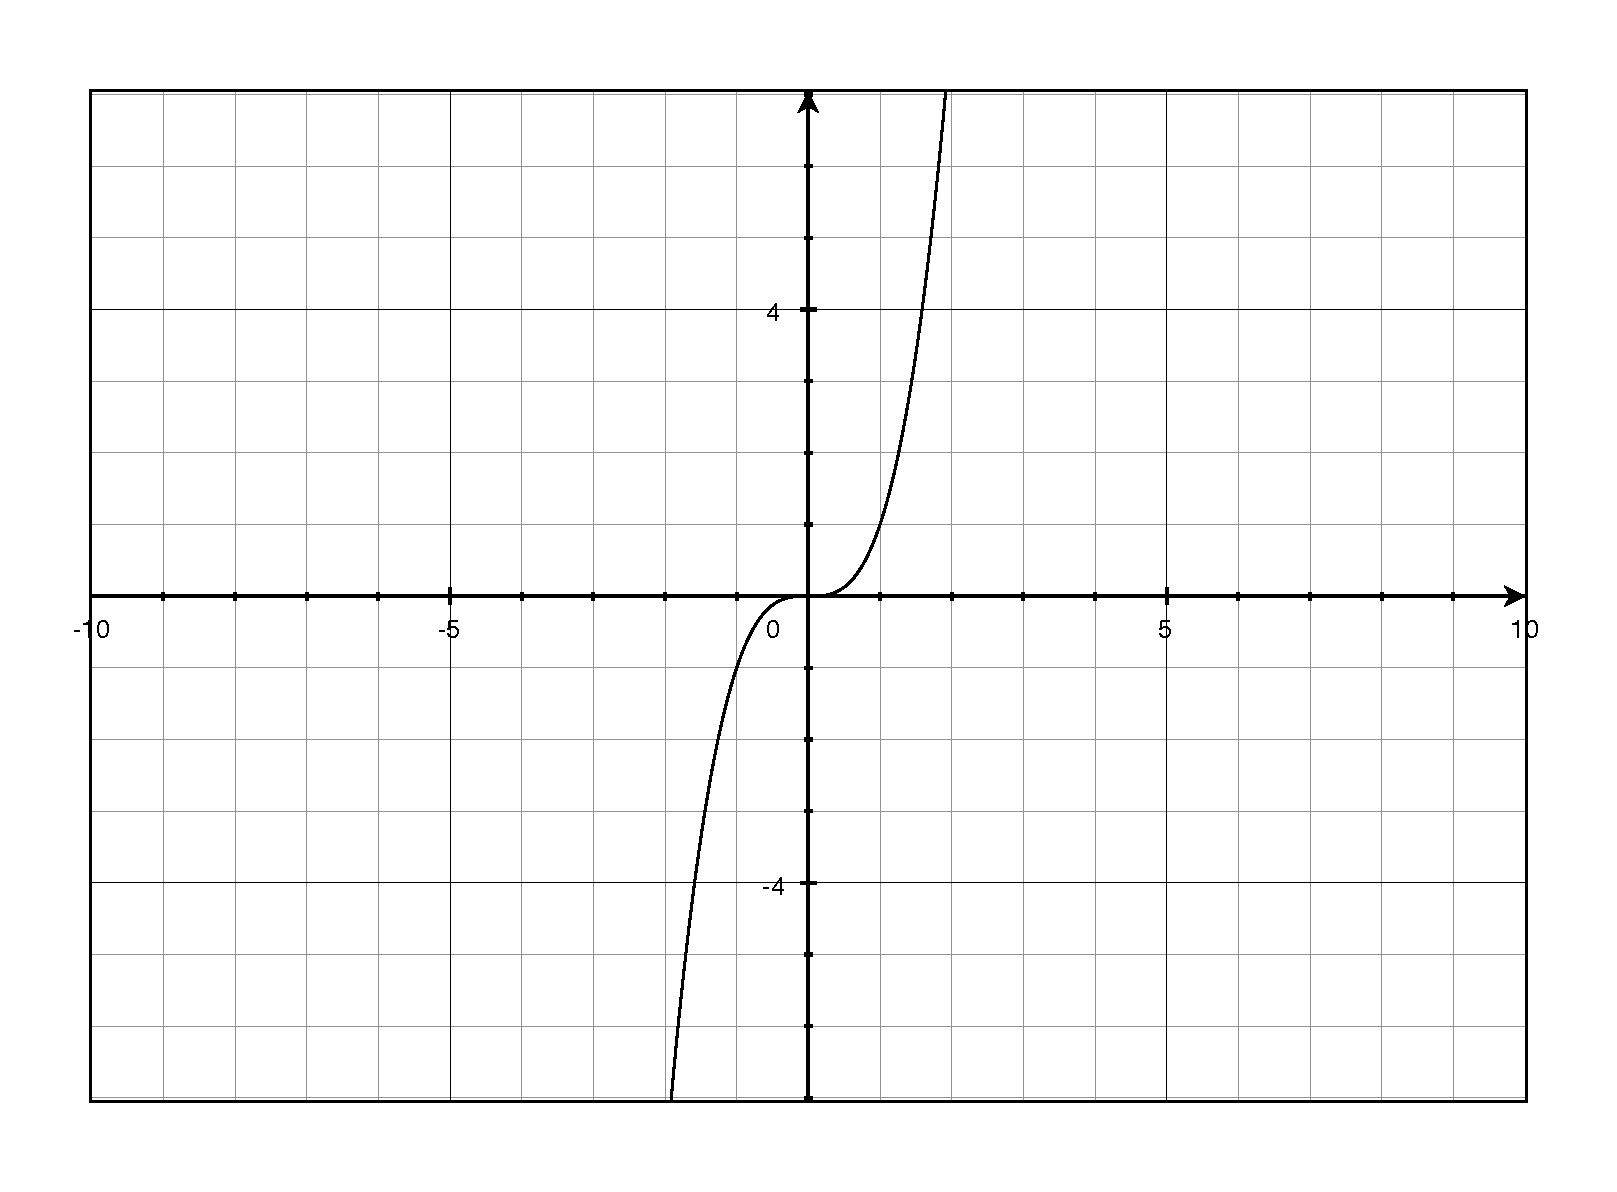
\includegraphics[width=7cm,height=5cm]{x3}
  \caption{$f(x) = x^3$}
\end{figure}
\end{center}

\begin{parts}

\part
\begin{center}
\begin{figure}[H]
  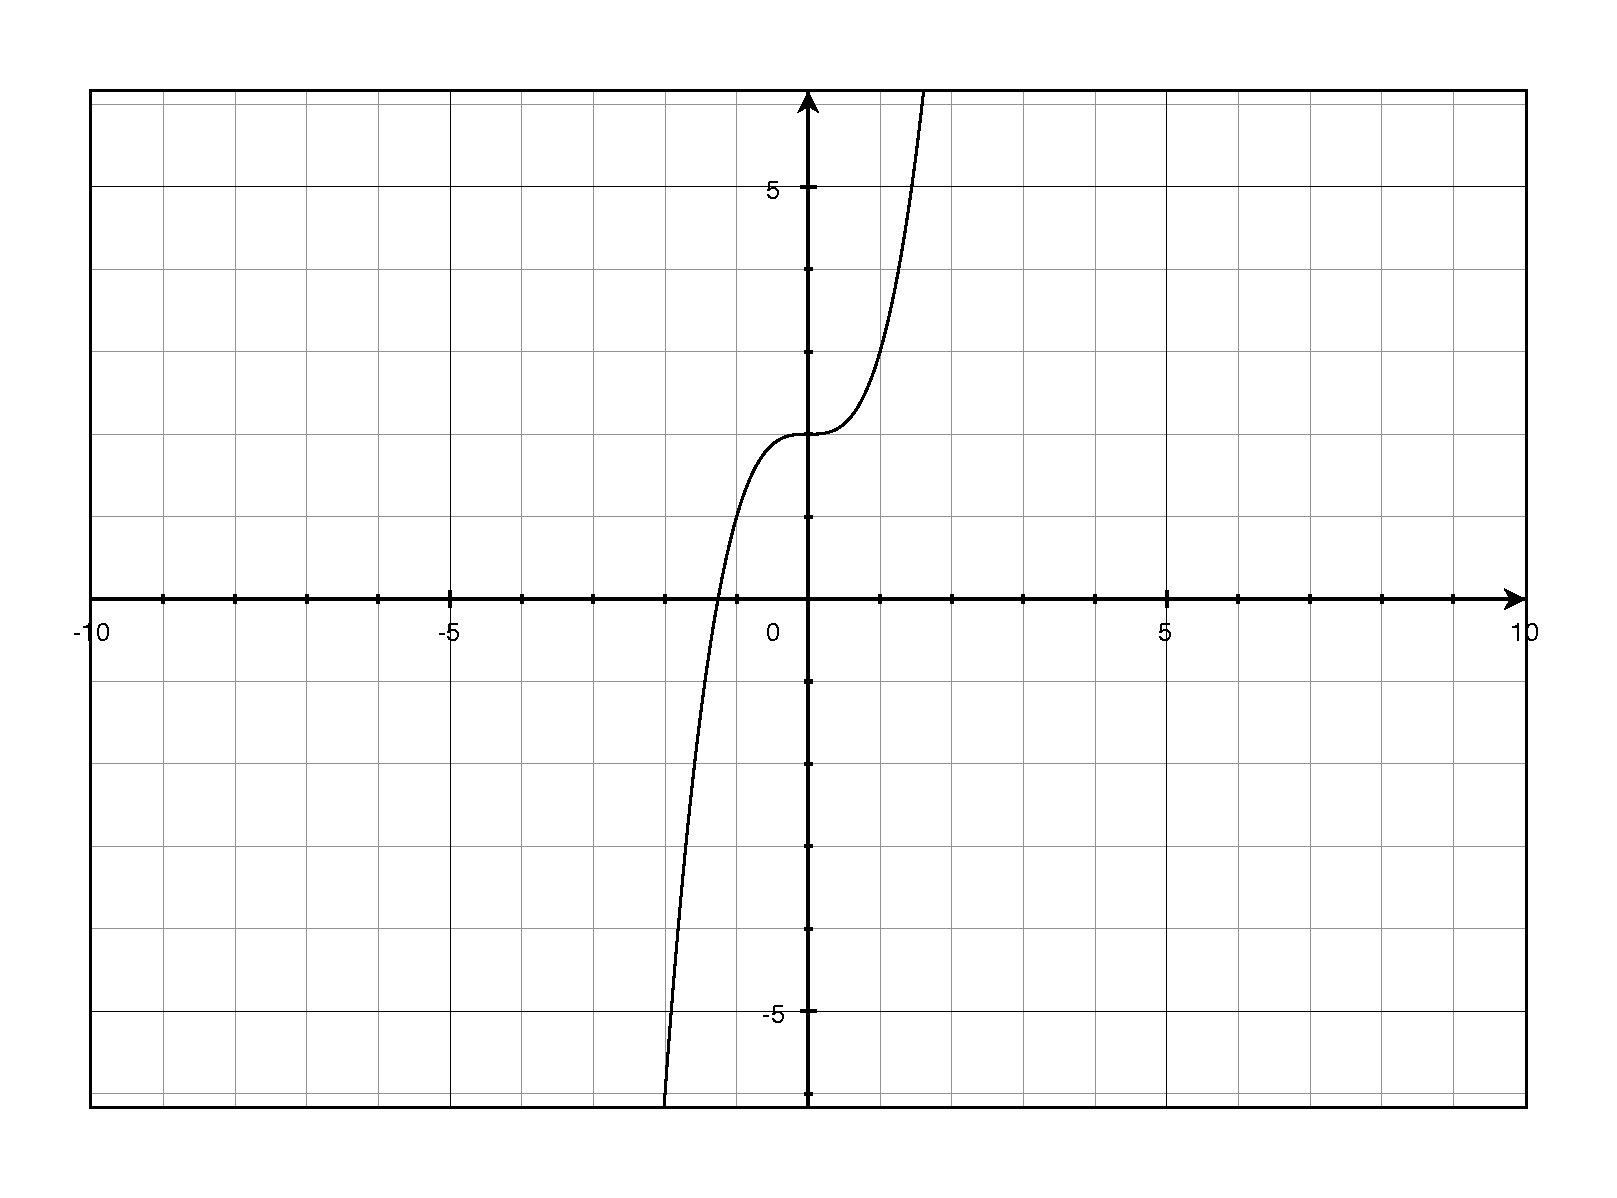
\includegraphics[width=7cm,height=5cm]{x3-a}
\end{figure}
\end{center}

\part
\begin{figure}[H]
  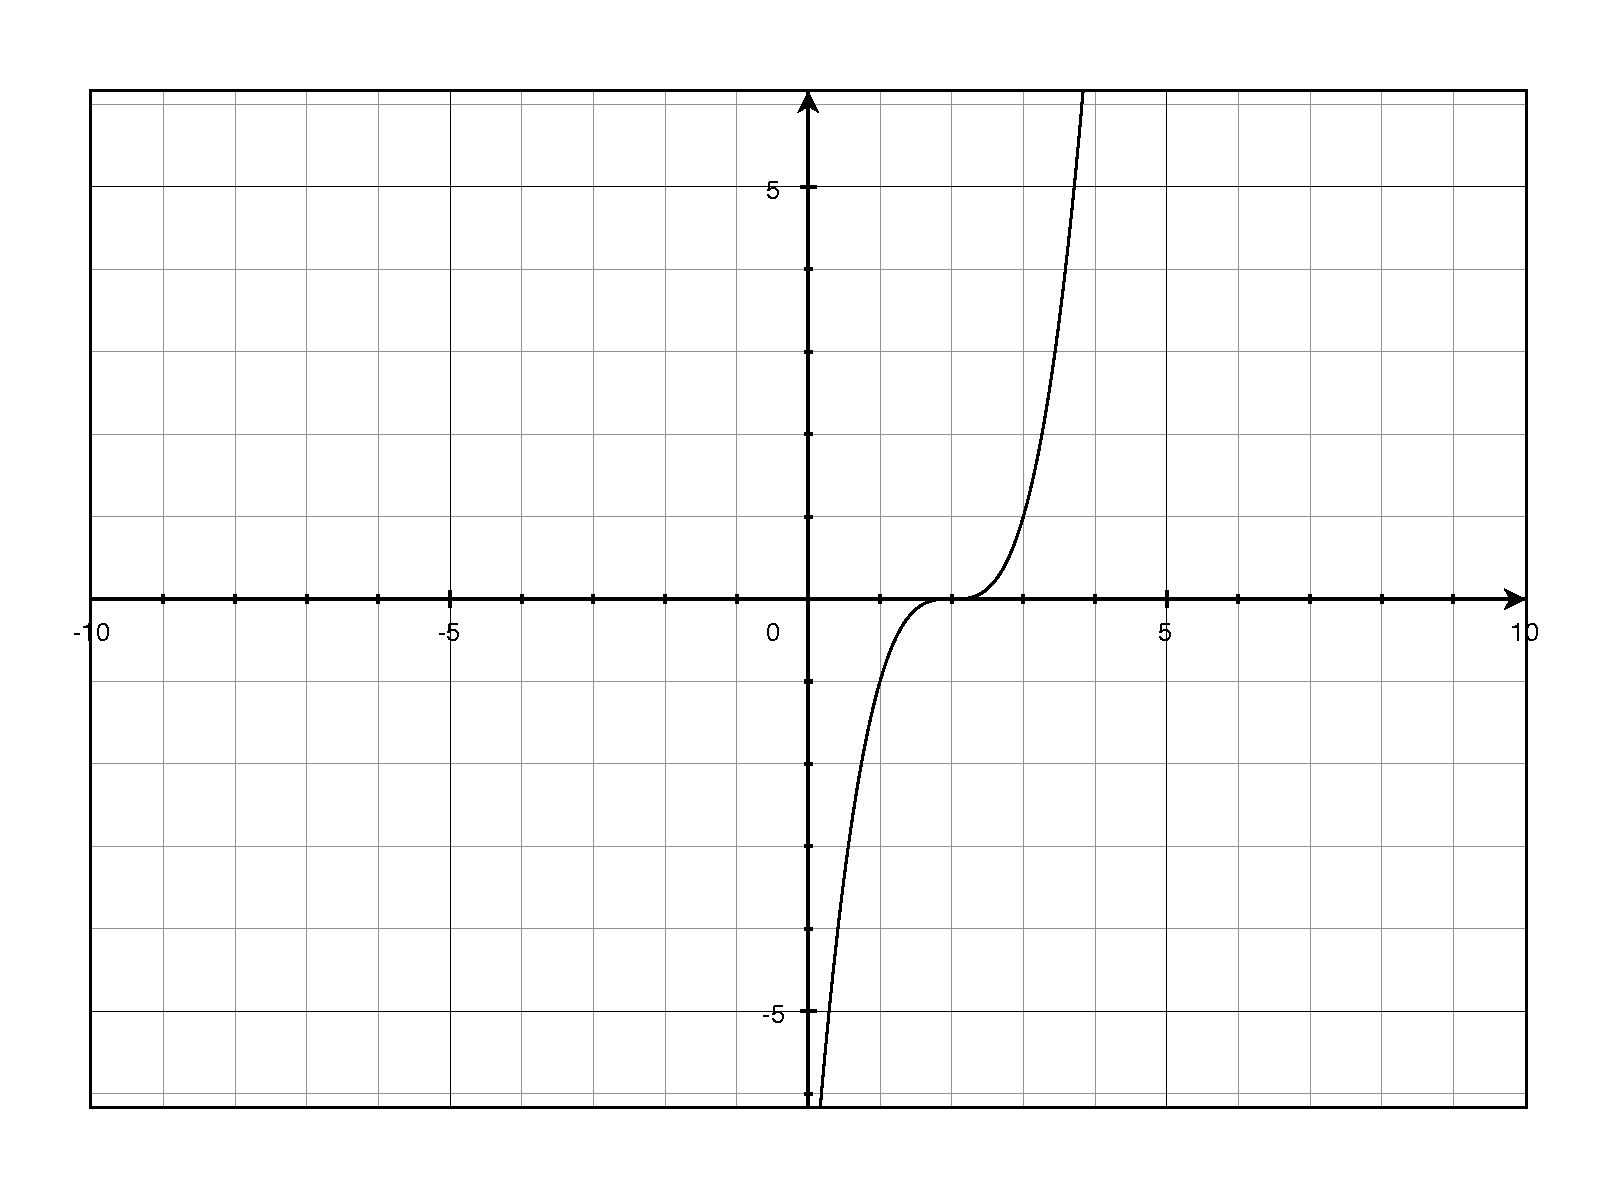
\includegraphics[width=7cm,height=5cm]{x3-b}
\end{figure}

\part
\begin{figure}[H]
  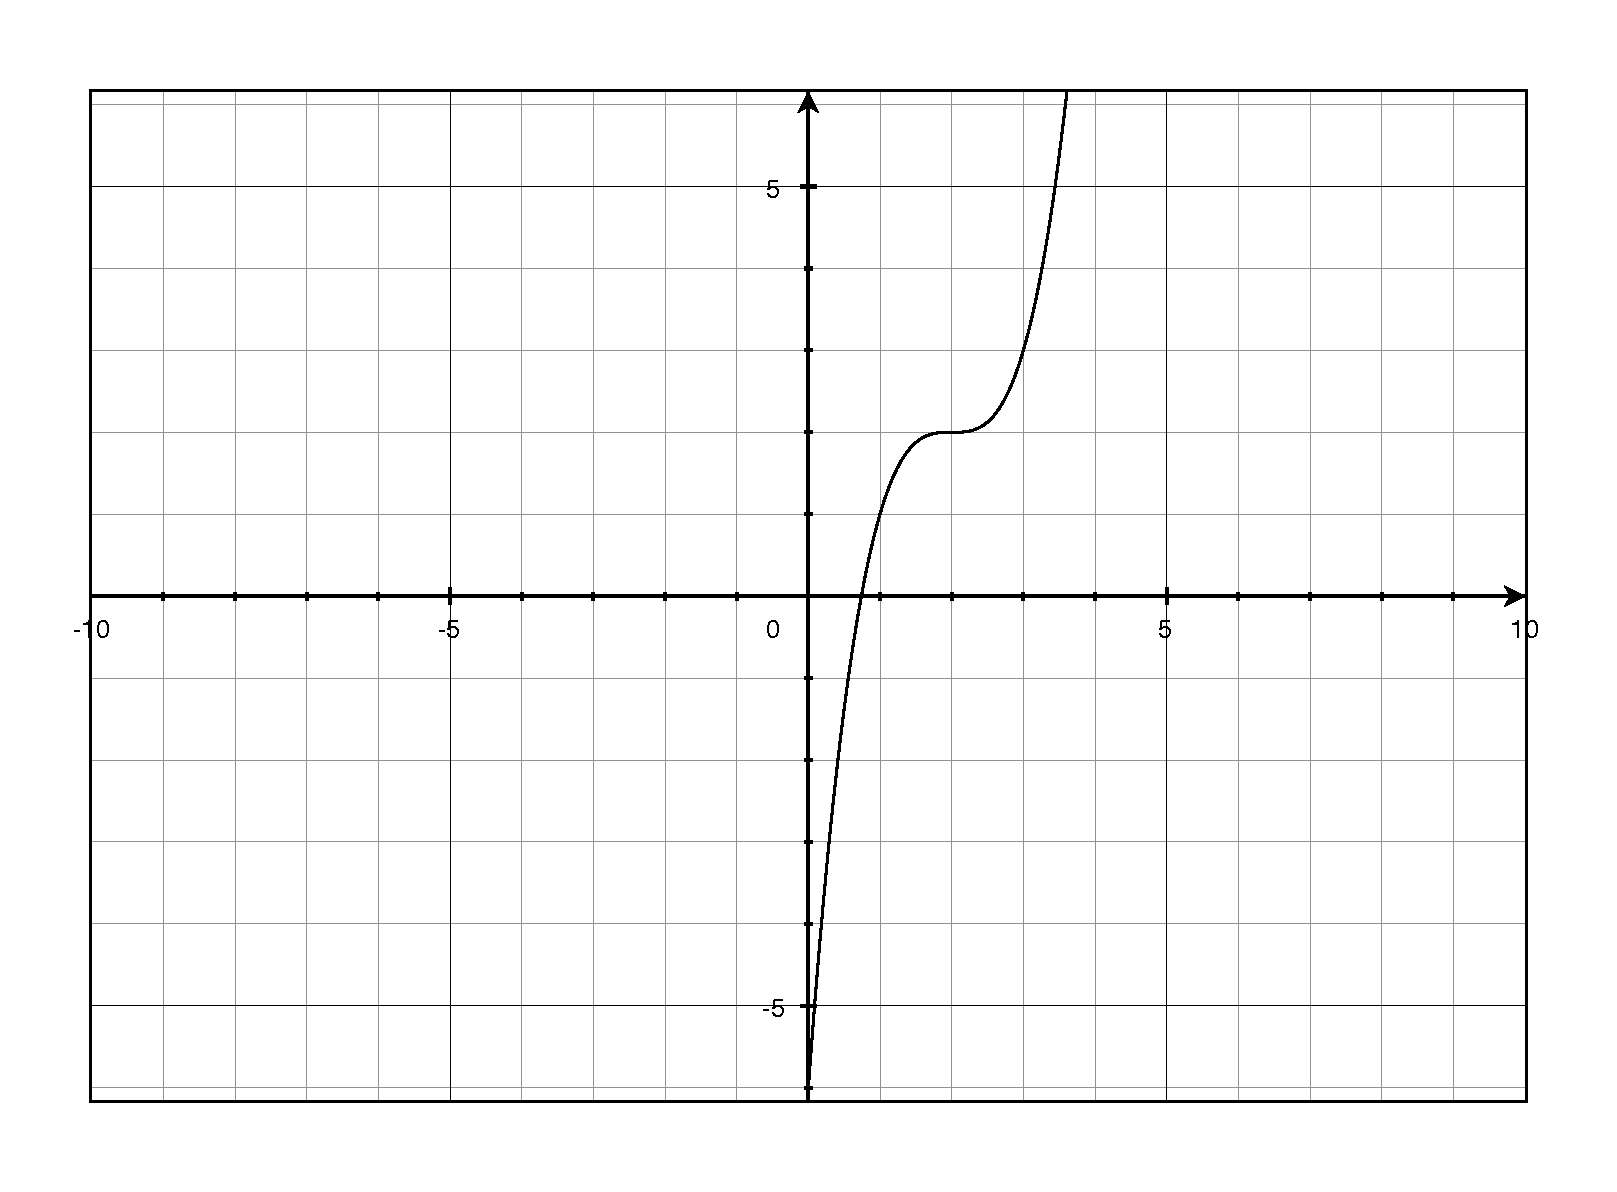
\includegraphics[width=7cm,height=5cm]{x3-c}
\end{figure}

\part
\begin{figure}[H]
  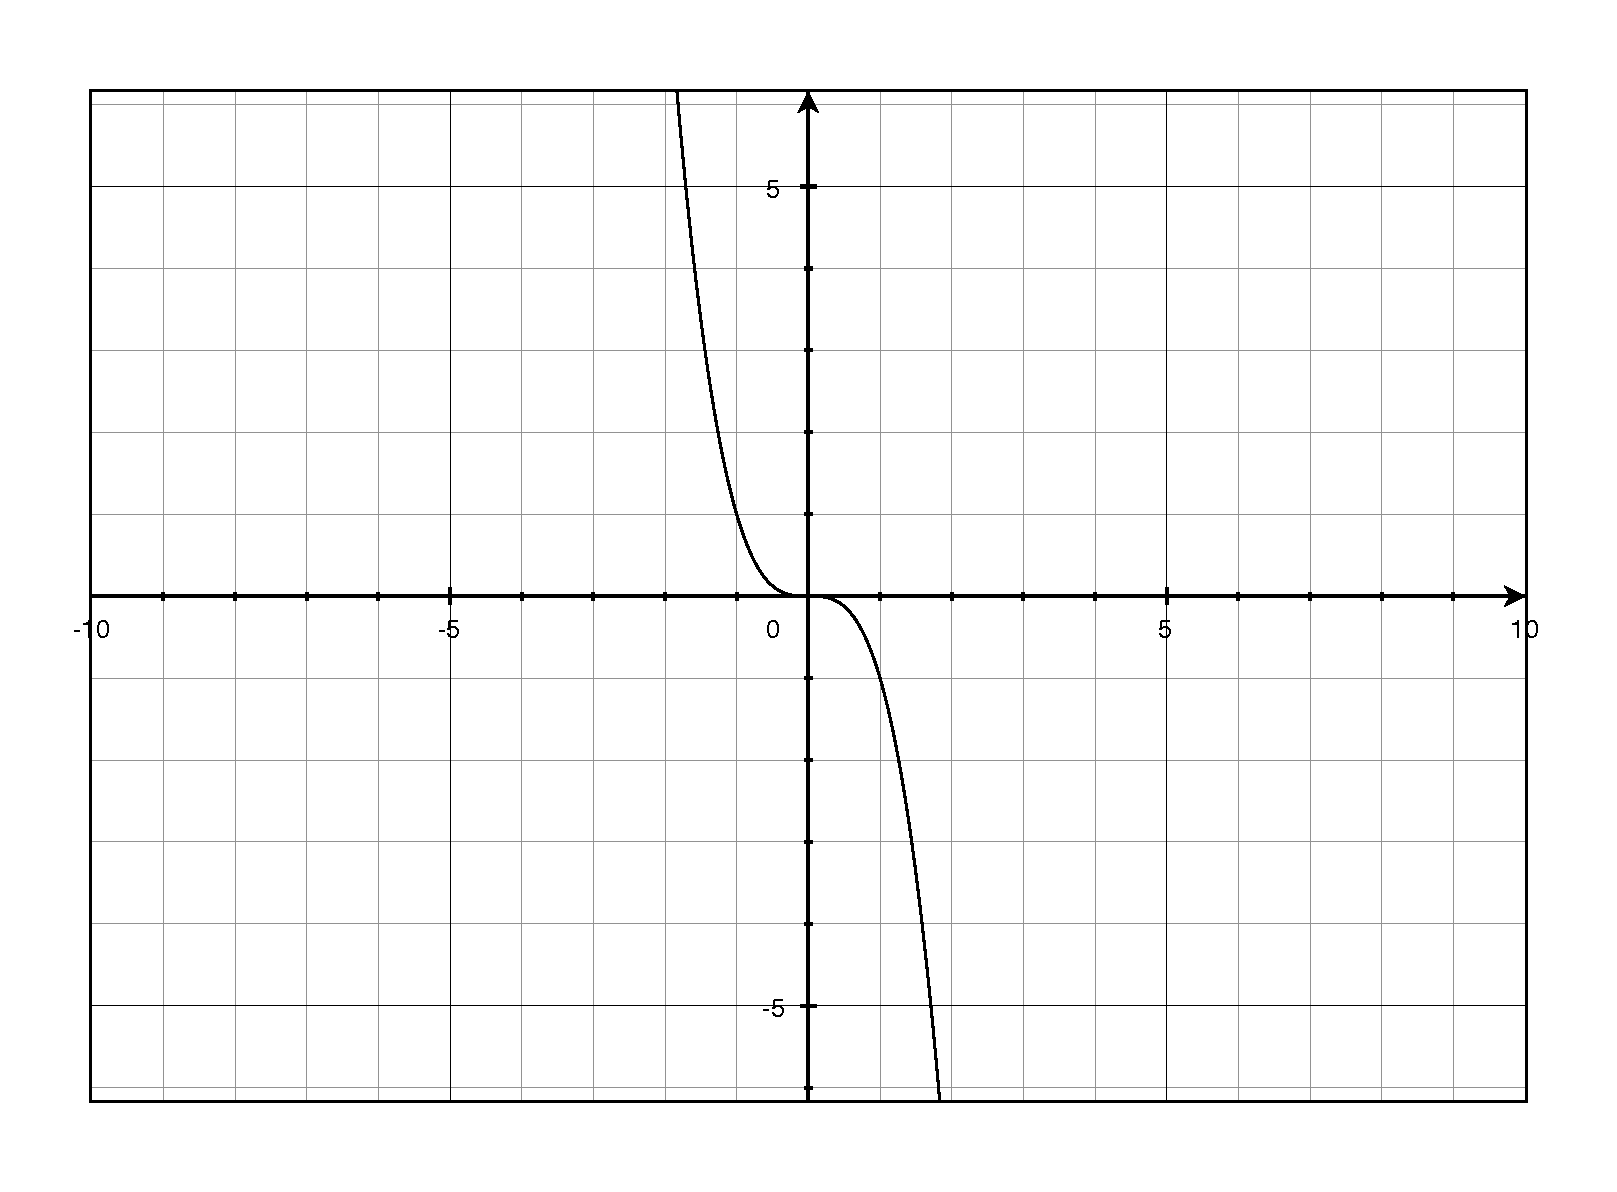
\includegraphics[width=7cm,height=5cm]{x3-d}
\end{figure}

\end{parts}

\pagebreak

\section{Quadratic Functions}

\question 
$f(x) = (x-1) + 3$

\begin{parts}
\part Where is the vertex?
\vspace{1cm}

\part Does the parabola open up or down?
\vspace{1cm}

\part
Draw the graph of this function.
\begin{figure}[H]
  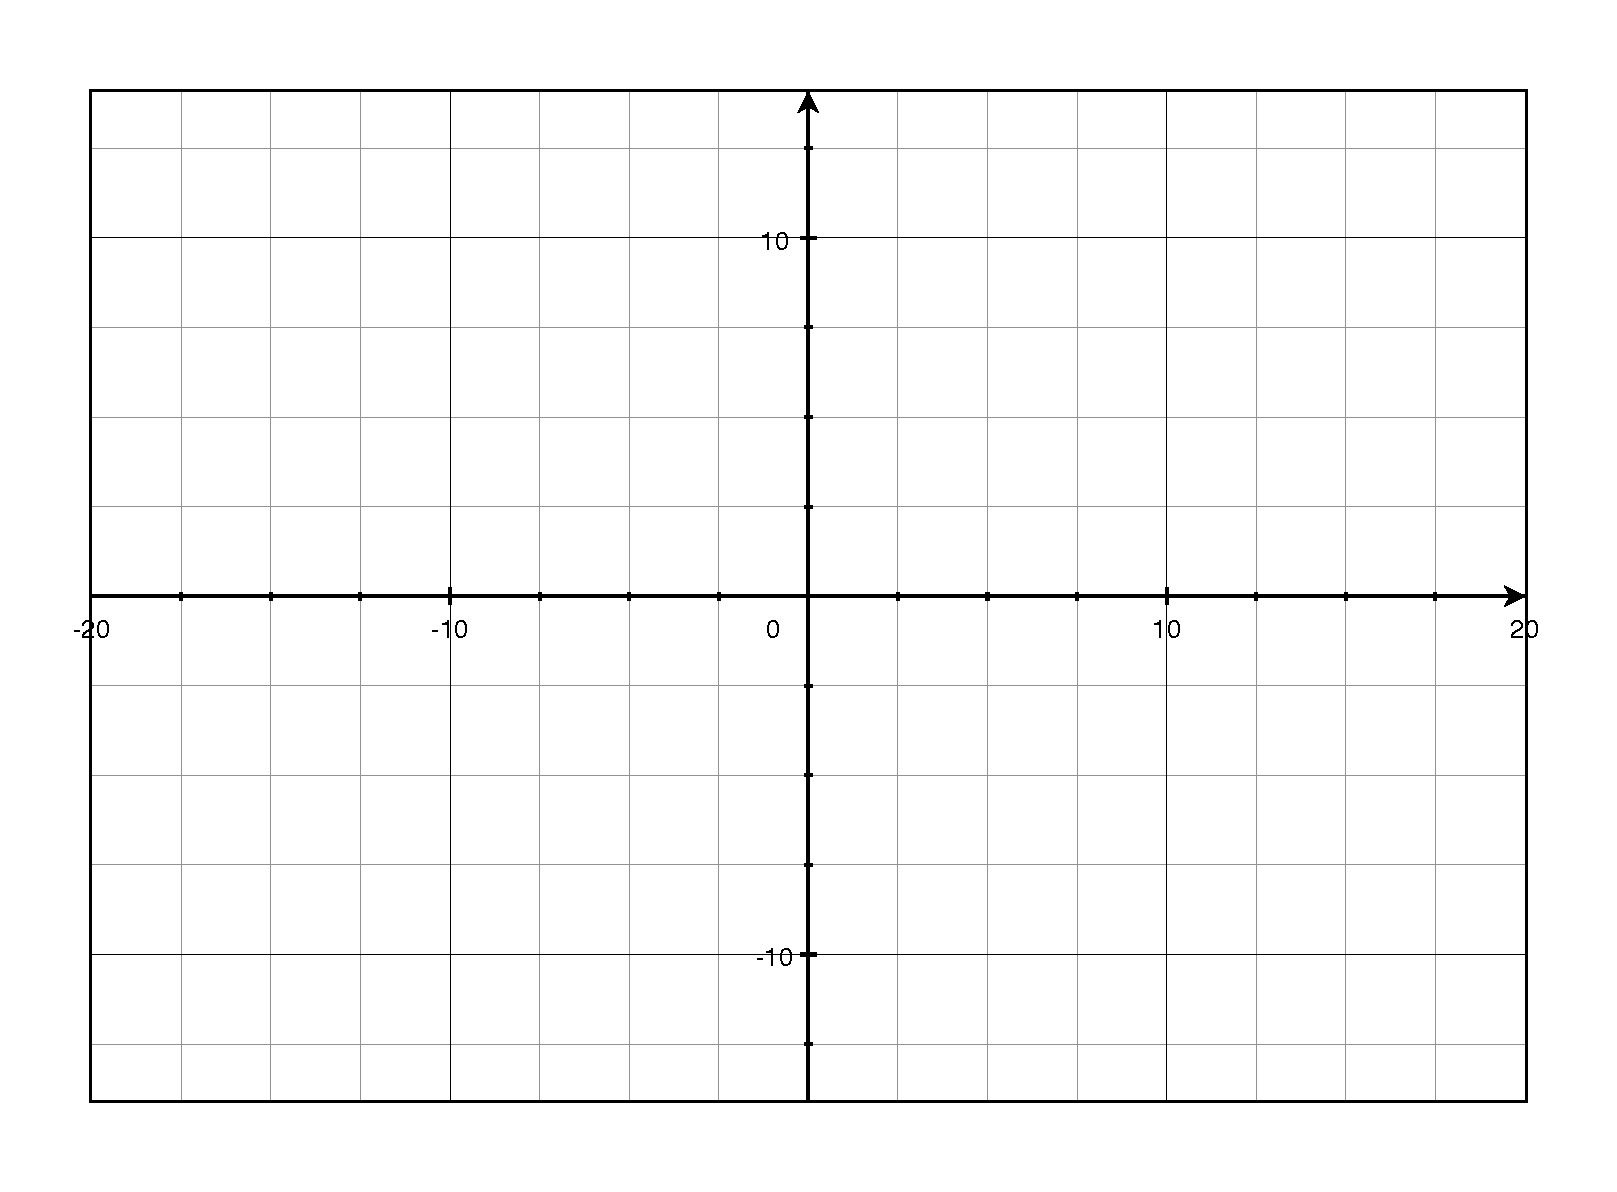
\includegraphics[width=7cm,height=5cm]{axes}
\end{figure}

\end{parts}

\question 
$f(x) = -x^2+2x-5$

\begin{parts}
\part Where is the vertex?
\vspace{2cm}

\part Does the parabola open up or down?
\vspace{1cm}

\part
Draw the graph of this function.
\begin{figure}[H]
  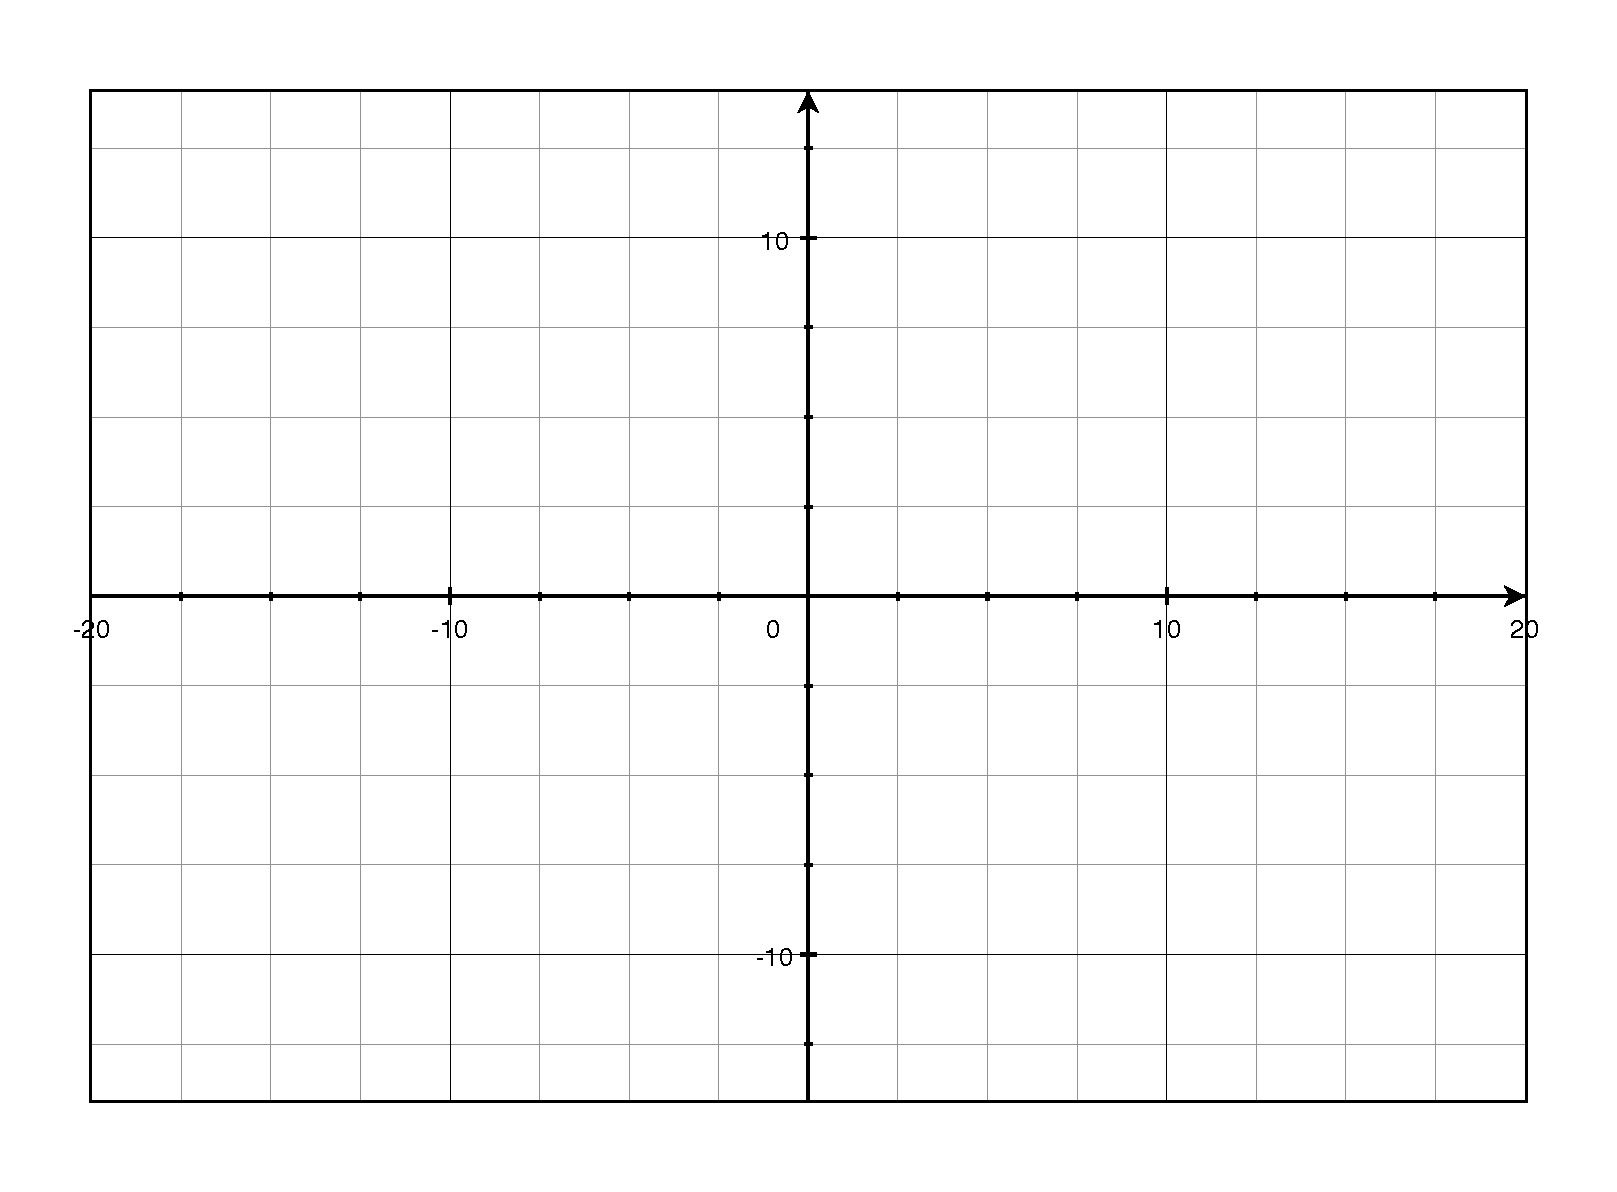
\includegraphics[width=7cm,height=5cm]{axes}
\end{figure}


\end{parts}

\end{questions}

\end{document}
